\documentclass{standalone}
\usepackage{tikz}
\usetikzlibrary{patterns, positioning}

\begin{document}
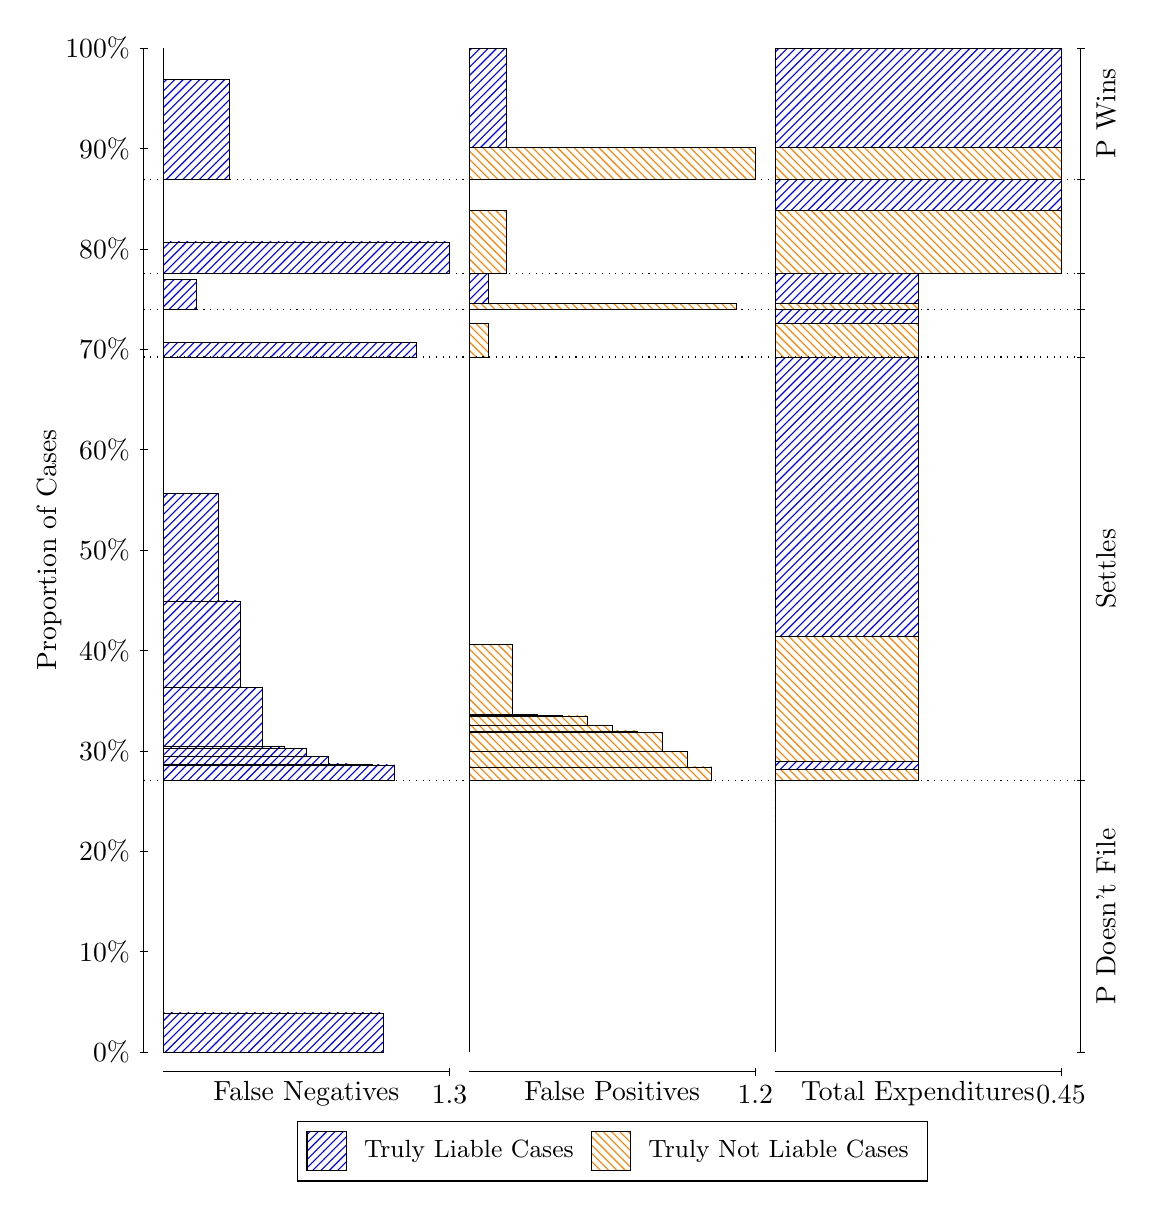
\begin{tikzpicture}
\draw[black, very thin] (1.5,1.75) -- (1.5,14.5);
\node[rotate=90, anchor=center] at (0.3, 8.125) {Proportion of Cases};
\draw[black, very thin] (1.45,1.75) -- (1.55,1.75);
\node[anchor=east] at (1.45, 1.75) {0\%};
\draw[black, very thin] (1.45,3.025) -- (1.55,3.025);
\node[anchor=east] at (1.45, 3.025) {10\%};
\draw[black, very thin] (1.45,4.3) -- (1.55,4.3);
\node[anchor=east] at (1.45, 4.3) {20\%};
\draw[black, very thin] (1.45,5.575) -- (1.55,5.575);
\node[anchor=east] at (1.45, 5.575) {30\%};
\draw[black, very thin] (1.45,6.85) -- (1.55,6.85);
\node[anchor=east] at (1.45, 6.85) {40\%};
\draw[black, very thin] (1.45,8.125) -- (1.55,8.125);
\node[anchor=east] at (1.45, 8.125) {50\%};
\draw[black, very thin] (1.45,9.4) -- (1.55,9.4);
\node[anchor=east] at (1.45, 9.4) {60\%};
\draw[black, very thin] (1.45,10.675) -- (1.55,10.675);
\node[anchor=east] at (1.45, 10.675) {70\%};
\draw[black, very thin] (1.45,11.95) -- (1.55,11.95);
\node[anchor=east] at (1.45, 11.95) {80\%};
\draw[black, very thin] (1.45,13.225) -- (1.55,13.225);
\node[anchor=east] at (1.45, 13.225) {90\%};
\draw[black, very thin] (1.45,14.5) -- (1.55,14.5);
\node[anchor=east] at (1.45, 14.5) {100\%};

\draw[black, very thin] (13.4,1.75) -- (13.4,14.5);
\draw[black, very thin] (13.35,1.75) -- (13.45,1.75);
\node[anchor=west] at (13.35, 1.75) {};
\draw[black, very thin] (13.35,5.1954) -- (13.45,5.1954);
\node[anchor=west] at (13.35, 5.1954) {};
\draw[black, very thin] (13.35,10.576) -- (13.45,10.576);
\node[anchor=west] at (13.35, 10.576) {};
\draw[black, very thin] (13.35,11.181) -- (13.45,11.181);
\node[anchor=west] at (13.35, 11.181) {};
\draw[black, very thin] (13.35,11.641) -- (13.45,11.641);
\node[anchor=west] at (13.35, 11.641) {};
\draw[black, very thin] (13.35,12.835) -- (13.45,12.835);
\node[anchor=west] at (13.35, 12.835) {};
\draw[black, very thin] (13.35,14.5) -- (13.45,14.5);
\node[anchor=west] at (13.35, 14.5) {};

\draw[black, very thin, pattern color=blue, pattern=north east lines] (1.75,1.75) rectangle (4.5449,2.2472);
\draw[black, very thin, pattern color=orange, pattern=north west lines] (1.75,2.2472) rectangle (1.75,5.1954);
\draw[black, very thin, pattern color=blue, pattern=north east lines] (1.75,5.1954) rectangle (4.6846,5.3971);
\draw[black, very thin, pattern color=blue, pattern=north east lines] (1.75,5.3971) rectangle (4.4051,5.4043);
\draw[black, very thin, pattern color=blue, pattern=north east lines] (1.75,5.4043) rectangle (4.1256,5.4098);
\draw[black, very thin, pattern color=blue, pattern=north east lines] (1.75,5.4098) rectangle (3.8462,5.502);
\draw[black, very thin, pattern color=blue, pattern=north east lines] (1.75,5.502) rectangle (3.5667,5.606);
\draw[black, very thin, pattern color=blue, pattern=north east lines] (1.75,5.606) rectangle (3.2872,5.6324);
\draw[black, very thin, pattern color=blue, pattern=north east lines] (1.75,5.6324) rectangle (3.0077,6.3767);
\draw[black, very thin, pattern color=blue, pattern=north east lines] (1.75,6.3767) rectangle (2.7282,7.4786);
\draw[black, very thin, pattern color=blue, pattern=north east lines] (1.75,7.4786) rectangle (2.4487,8.8475);
\draw[black, very thin, pattern color=orange, pattern=north west lines] (1.75,8.8475) rectangle (1.75,10.576);
\draw[black, very thin, pattern color=blue, pattern=north east lines] (1.75,10.576) rectangle (4.9641,10.757);
\draw[black, very thin, pattern color=orange, pattern=north west lines] (1.75,10.757) rectangle (1.75,11.181);
\draw[black, very thin, pattern color=blue, pattern=north east lines] (1.75,11.181) rectangle (2.1692,11.564);
\draw[black, very thin, pattern color=orange, pattern=north west lines] (1.75,11.564) rectangle (1.75,11.641);
\draw[black, very thin, pattern color=blue, pattern=north east lines] (1.75,11.641) rectangle (5.3833,12.039);
\draw[black, very thin, pattern color=orange, pattern=north west lines] (1.75,12.039) rectangle (1.75,12.835);
\draw[black, very thin, pattern color=blue, pattern=north east lines] (1.75,12.835) rectangle (2.5885,14.1);
\draw[black, very thin, pattern color=orange, pattern=north west lines] (1.75,14.1) rectangle (1.75,14.5);
\draw[black, very thin, pattern color=orange, pattern=north west lines] (5.6333,1.75) rectangle (5.6333,4.6982);
\draw[black, very thin, pattern color=blue, pattern=north east lines] (5.6333,4.6982) rectangle (5.6333,5.1954);
\draw[black, very thin, pattern color=orange, pattern=north west lines] (5.6333,5.1954) rectangle (8.7138,5.3701);
\draw[black, very thin, pattern color=orange, pattern=north west lines] (5.6333,5.3701) rectangle (8.3978,5.5656);
\draw[black, very thin, pattern color=orange, pattern=north west lines] (5.6333,5.5656) rectangle (8.0819,5.8099);
\draw[black, very thin, pattern color=orange, pattern=north west lines] (5.6333,5.8099) rectangle (7.7659,5.8285);
\draw[black, very thin, pattern color=orange, pattern=north west lines] (5.6333,5.8285) rectangle (7.45,5.8972);
\draw[black, very thin, pattern color=orange, pattern=north west lines] (5.6333,5.8972) rectangle (7.1341,5.8976);
\draw[black, very thin, pattern color=orange, pattern=north west lines] (5.6333,5.8976) rectangle (7.1341,6.0169);
\draw[black, very thin, pattern color=orange, pattern=north west lines] (5.6333,6.0169) rectangle (6.8181,6.0222);
\draw[black, very thin, pattern color=orange, pattern=north west lines] (5.6333,6.0222) rectangle (6.5022,6.0393);
\draw[black, very thin, pattern color=orange, pattern=north west lines] (5.6333,6.0393) rectangle (6.1862,6.9242);
\draw[black, very thin, pattern color=blue, pattern=north east lines] (5.6333,6.9242) rectangle (5.6333,10.576);
\draw[black, very thin, pattern color=orange, pattern=north west lines] (5.6333,10.576) rectangle (5.8703,11.001);
\draw[black, very thin, pattern color=blue, pattern=north east lines] (5.6333,11.001) rectangle (5.6333,11.181);
\draw[black, very thin, pattern color=orange, pattern=north west lines] (5.6333,11.181) rectangle (9.0297,11.258);
\draw[black, very thin, pattern color=blue, pattern=north east lines] (5.6333,11.258) rectangle (5.8703,11.641);
\draw[black, very thin, pattern color=orange, pattern=north west lines] (5.6333,11.641) rectangle (6.1072,12.438);
\draw[black, very thin, pattern color=blue, pattern=north east lines] (5.6333,12.438) rectangle (5.6333,12.835);
\draw[black, very thin, pattern color=orange, pattern=north west lines] (5.6333,12.835) rectangle (9.2667,13.235);
\draw[black, very thin, pattern color=blue, pattern=north east lines] (5.6333,13.235) rectangle (6.1072,14.5);
\draw[black, very thin, pattern color=orange, pattern=north west lines] (9.5167,1.75) rectangle (9.5167,4.6982);
\draw[black, very thin, pattern color=blue, pattern=north east lines] (9.5167,4.6982) rectangle (9.5167,5.1954);
\draw[black, very thin, pattern color=orange, pattern=north west lines] (9.5167,5.1954) rectangle (11.333,5.1959);
\draw[black, very thin, pattern color=blue, pattern=north east lines] (9.5167,5.1959) rectangle (11.333,5.1965);
\draw[black, very thin, pattern color=orange, pattern=north west lines] (9.5167,5.1965) rectangle (11.333,5.3381);
\draw[black, very thin, pattern color=blue, pattern=north east lines] (9.5167,5.3381) rectangle (11.333,5.4425);
\draw[black, very thin, pattern color=orange, pattern=north west lines] (9.5167,5.4425) rectangle (11.333,7.0292);
\draw[black, very thin, pattern color=blue, pattern=north east lines] (9.5167,7.0292) rectangle (11.333,10.576);
\draw[black, very thin, pattern color=orange, pattern=north west lines] (9.5167,10.576) rectangle (11.333,11.001);
\draw[black, very thin, pattern color=blue, pattern=north east lines] (9.5167,11.001) rectangle (11.333,11.181);
\draw[black, very thin, pattern color=orange, pattern=north west lines] (9.5167,11.181) rectangle (11.333,11.258);
\draw[black, very thin, pattern color=blue, pattern=north east lines] (9.5167,11.258) rectangle (11.333,11.641);
\draw[black, very thin, pattern color=orange, pattern=north west lines] (9.5167,11.641) rectangle (13.15,12.438);
\draw[black, very thin, pattern color=blue, pattern=north east lines] (9.5167,12.438) rectangle (13.15,12.835);
\draw[black, very thin, pattern color=orange, pattern=north west lines] (9.5167,12.835) rectangle (13.15,13.235);
\draw[black, very thin, pattern color=blue, pattern=north east lines] (9.5167,13.235) rectangle (13.15,14.5);
\draw[black, dotted] (1.5,5.1954) -- (13.4,5.1954);
\draw[black, dotted] (1.5,10.576) -- (13.4,10.576);
\draw[black, dotted] (1.5,11.181) -- (13.4,11.181);
\draw[black, dotted] (1.5,11.641) -- (13.4,11.641);
\draw[black, dotted] (1.5,12.835) -- (13.4,12.835);
\draw[black, very thin] (1.75,1.5) -- (5.3833,1.5);
\node[anchor=north] at (3.5667, 1.5) {False Negatives};
\draw[black, very thin] (5.3833,1.45) -- (5.3833,1.55);
\node[anchor=north] at (5.3833, 1.45) {1.3};

\draw[black, very thin] (5.6333,1.5) -- (9.2667,1.5);
\node[anchor=north] at (7.45, 1.5) {False Positives};
\draw[black, very thin] (9.2667,1.45) -- (9.2667,1.55);
\node[anchor=north] at (9.2667, 1.45) {1.2};

\draw[black, very thin] (9.5167,1.5) -- (13.15,1.5);
\node[anchor=north] at (11.333, 1.5) {Total Expenditures};
\draw[black, very thin] (13.15,1.45) -- (13.15,1.55);
\node[anchor=north] at (13.15, 1.45) {0.45};

\node[black, centered, rotate=90] at (13.72, 3.4727) {P Doesn't File};
\node[black, centered, rotate=90] at (13.72, 7.8859) {Settles};



\node[black, centered, rotate=90] at (13.72, 13.668) {P Wins};

\draw (7.449999999999999,1.5) node[draw=none] (baseCoordinate) {};
\begin{scope}[align=center]
        \matrix[scale=0.5, draw=black, below=0.5cm of baseCoordinate, nodes={draw}, column sep=0.1cm]{
            \node[rectangle, draw, minimum width=0.5cm, minimum height=0.5cm, pattern=north east lines, pattern color=blue] {}; &
            \node[draw=none, font=\small] (B) {Truly Liable Cases}; &
            \node[rectangle, draw, minimum width=0.5cm, minimum height=0.5cm, pattern=north west lines, pattern color=orange] {}; &
            \node[draw=none, font=\small] (B) {Truly Not Liable Cases}; \\
            };
\end{scope}

\end{tikzpicture}
\end{document}